\chapter{측지선, 등가속도, 뉴턴 역학의 극한}

당면한 문제는 중력이다. 더 정확히 말해, 지구 표면 근처의 작은 실험실 안에서처럼 거의 균일한 중력장을 나타내는 시공간 계량을 구하고자 한다. 그 계량을 얻는 가장 빠른 길은 곧장 나아가는 길이 아니다. 먼저 세 가지 기하학적 개념을 실제로 적용할 수 있게 정식화해야 한다. 공변미분, 평행이동, 측지선 운동이 그것이다.

이 개념들은 서로 의존한다. 공변미분은 서로 이웃한 점에 있는 벡터를 어떻게 비교할지 알려 준다. 평행이동은 벡터의 방향을 바꾸지 않고 옮기는 방법을 알려 준다. 옮기는 벡터가 경로 자체의 접벡터일 때 측지선이 얻어진다. 경로가 공간이 아니라 시공간에 놓이면, 같은 측지선 방정식이 자유낙하 입자의 운동 방정식이 된다.

이어서 강의의 후반부에서는 놀라운 전환이 이루어진다. 평탄한 민코프스키 시공간에 머물면서 강체 가속 관측자 무리에 맞춘 좌표로 시공간을 기술한다. 이 좌표에서 계량은 중력장이 있는 것처럼 보인다. 한 관측자 근방에서는 균일한 장의 퍼텐셜을 재현하고, 측지선은 뉴턴 역학의 방정식
\begin{equation}
\frac{d^2y}{d\tau^2}=-g.
\end{equation}
을 따른다. 이는 계산으로 표현한 등가원리다.

\section{공변미분 복습}

선택한 한 점 \(P\)에서 좌표를 가능한 한 데카르트 좌표에 가깝게 잡을 수 있다. 강의에서는 처음에 가우스 법선좌표라는 표현을 쓰지만, 곧바로 그 의미를 한정한다. 명칭보다 중요한 것은 그 점에서 성립하는 국소 조건이다.
\begin{equation}
g_{mn}(P)=\delta_{mn},
\qquad
\partial_r g_{mn}(P)=0.
\label{eq:l4-normal-point}
\end{equation}
이것은 한 점에서의 법선좌표다. 유한한 근방 전체에서 데카르트 좌표일 필요는 없으며, 좌표축을 회전할 수 있으므로 이러한 좌표계는 여러 개 존재한다.

계량은 미분 연산자와 양립한다.
\begin{equation}
\nabla_r g_{mn}=0,
\qquad
\nabla_r g^{mn}=0.
\label{eq:l4-metric-compatibility}
\end{equation}
공변벡터 \(V_s\)의 공변미분은 다음과 같다.
\begin{equation}
\nabla_r V_s
=
\partial_r V_s-\Gamma^p{}_{rs}V_p.
\label{eq:l4-covector-derivative}
\end{equation}
접속계수는 다음과 같다.
\begin{equation}
\Gamma^p{}_{rs}
=
\frac{1}{2}g^{pn}
\left(
\partial_s g_{nr}
+\partial_r g_{ns}
-\partial_n g_{rs}
\right).
\label{eq:l4-christoffel}
\end{equation}
이 식을 칠판에 쓰는 동안 몇몇 지표가 수정된다. \eqref{eq:l4-christoffel}은 완성된 관계식이다. 예상대로 비틀림이 없는 레비치비타 접속이므로 \(r\)와 \(s\)에 대해 대칭이다.

\begin{figure}[htbp]\centering
\includegraphics[width=0.92\textwidth]{lecture_04_figure_01.png}\caption{공변벡터의 미분과 완성된 크리스토펠 기호 공식.}\end{figure}

크리스토펠 기호는 계량의 1차 미분으로 만들어지므로, 좌표 \eqref{eq:l4-normal-point}에서는 \(P\)에서 사라진다. 하지만 바탕 공간이 평탄하더라도 모든 좌표계에서 사라지는 것은 아니다. 따라서 \(\Gamma^p{}_{rs}\)은 텐서가 아니다. 이 비텐서적 성질 덕분에 훗날 가속 관측자는 관성 관측자에게는 보이지 않는 중력력을 기술할 수 있다.

\subsection{벡터 지표 올리기}

벡터의 공변미분은 따로 외워야 하는 규칙으로 도입하지 않는다. 계량에서 유도된다. 다음 식에서 시작하자.
\begin{equation}
V^n=g^{np}V_p.
\end{equation}
그러면
\begin{align}
\nabla_m V^n
&=\nabla_m\!\left(g^{np}V_p\right) \\
&=(\nabla_m g^{np})V_p+g^{np}\nabla_m V_p \\
&=g^{np}\left(\partial_mV_p-\Gamma^r{}_{mp}V_r\right),
\end{align}
여기서는 계량의 양립성 때문에 첫째 항이 사라졌다. 지표를 다시 정리하면
\begin{equation}
\nabla_m V^n
=
\partial_m V^n+\Gamma^n{}_{mr}V^r.
\label{eq:l4-vector-derivative}
\end{equation}

\begin{figure}[htbp]\centering
\includegraphics[width=0.90\textwidth]{lecture_04_figure_02.png}\caption{미분하기 전에 역계량으로 지표를 올린다.}\end{figure}

\begin{figure}[htbp]\centering
\includegraphics[width=0.90\textwidth]{lecture_04_figure_03.png}\caption{계량의 양립성과 곱의 미분법에서 위 지표를 가진 공변미분이 나온다.}\end{figure}

따라서 지표에 따른 규칙은 간단하다.
\begin{equation}
\boxed{
\begin{aligned}
\text{lower index:}&\quad -\Gamma,\\
\text{upper index:}&\quad +\Gamma.
\end{aligned}}
\end{equation}
고차 텐서에서는 각 지표마다 접속 항이 하나씩 나타나며, 그 부호는 해당 지표가 아래에 있는지 위에 있는지에 따라 정해진다.

\subsection{용어에 관한 질문}

앞서 언급한 최적 좌표계란 정확히 무엇일까요? 특별한 전역 좌표계를 가리키는 것은 아닙니다. 선택한 한 점에서 계량을 평탄한 형태로 만들고 그 일차 미분을 영으로 만드는 좌표계입니다. 축을 회전해도 똑같이 적합한 좌표계가 됩니다. 그렇게 정한 좌표계에서 얻은 기하학적 진술은 축의 방향에 의존하지 않습니다. 최종적으로 얻는 대상이 텐서이기 때문입니다.

\section{곡선을 따른 평행이동}

벡터 \(V^n\)를 곡선을 따라 옮긴다고 하자. 무한소 변위 \(dx^m\)에 따른 벡터의 공변 변화는
\begin{align}
\delta V^n
&=(\nabla_mV^n)\,dx^m \\
&=\partial_mV^n\,dx^m
+\Gamma^n{}_{mr}V^r\,dx^m \\
&=dV^n+\Gamma^n{}_{mr}V^r\,dx^m.
\label{eq:l4-covariant-differential}
\end{align}

\begin{figure}[htbp]\centering
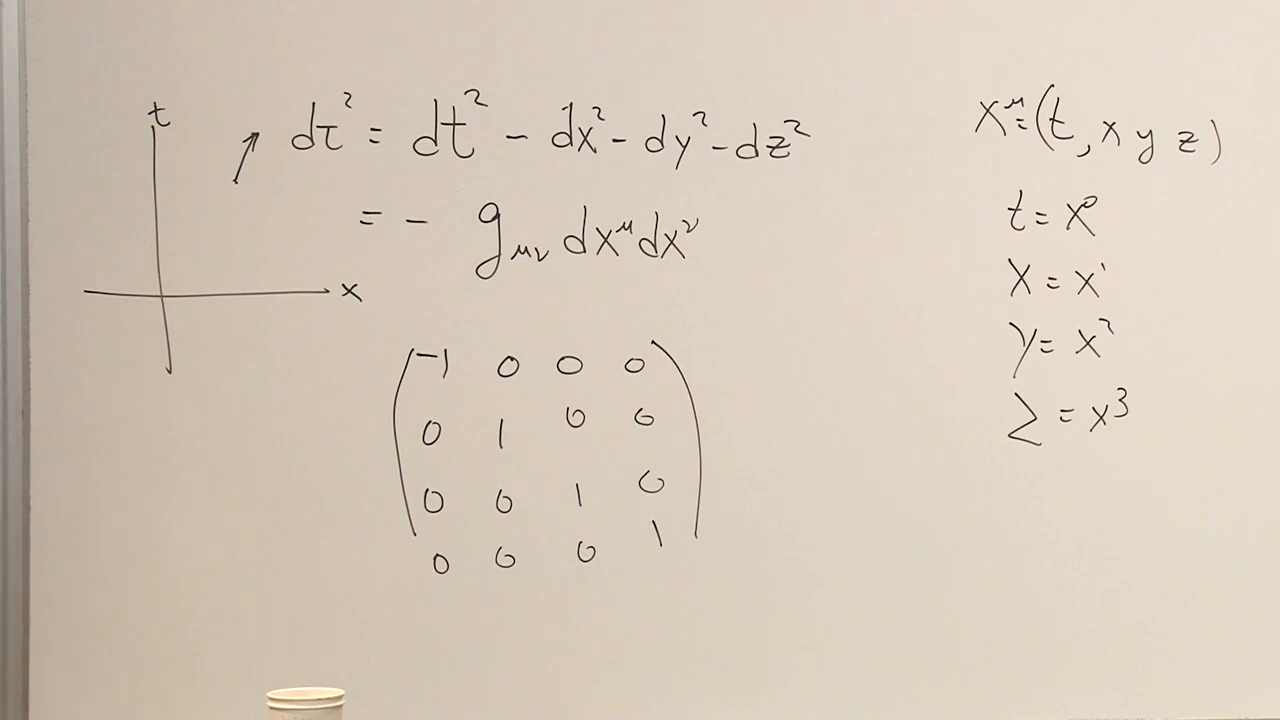
\includegraphics[width=0.92\textwidth]{lecture_04_figure_04.png}\caption{곡선을 따라 일어나는 성분의 일반 변화와 접속 보정.}\end{figure}

다음 공변 변화가 영일 때 벡터는 평행 이동됩니다:
\begin{equation}
\boxed{
dV^n+\Gamma^n{}_{mr}V^r\,dx^m=0.
}
\label{eq:l4-parallel-transport}
\end{equation}
이를 실제로 구현하는 방법으로는 곡선의 각 점에 국소 관성계를 세운다고 생각할 수 있습니다. 그 국소 좌표계에서 이동하는 벡터는 회전하지 않아야 합니다. 그런 다음 무한소 거리만큼 이동하고, 다음 국소 관성계를 세운 뒤 같은 과정을 반복합니다.

\begin{figure}[htbp]\centering
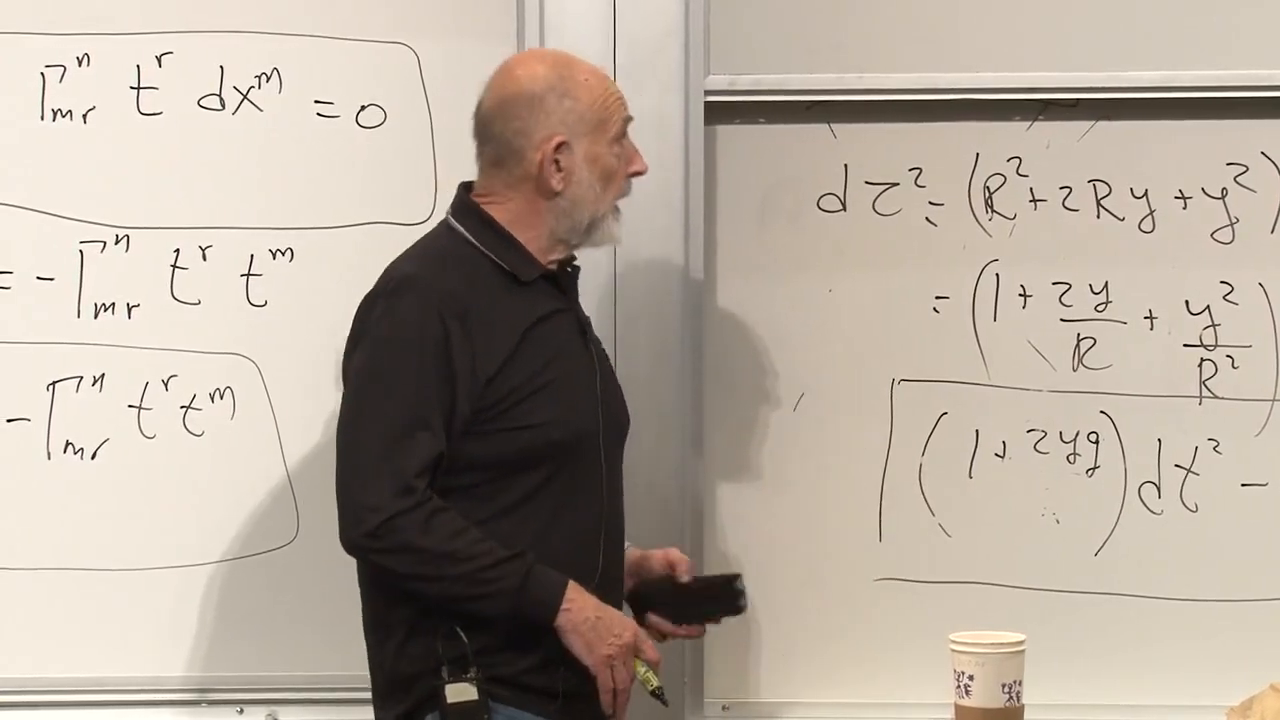
\includegraphics[width=0.92\textwidth]{lecture_04_figure_05.png}\caption{평행이동 방정식이 명확히 정리된 칠판 상태.}\end{figure}

각 임시 법선좌표계의 방향은 물리와 무관하다. 비교하기 전에 좌표계를 회전해도 된다. 중요한 것은 공변적 진술 \eqref{eq:l4-parallel-transport}이 그런 임의의 선택과 무관하다는 점이다.

\subsection{경로 의존성과 곡률}

곡률이 있는 공간에서는 평행이동 결과가 경로에 따라 달라진다. 같은 시작점에서 같은 벡터를 택해 서로 다른 두 경로를 따라 같은 끝점까지 옮겨 보자. 일반적으로 마지막 벡터들은 서로 다르다. 벡터를 닫힌 경로를 따라 옮기면 회전된 상태로 돌아올 수 있다. 이 차이를 홀로노미라 하며, 곡률을 직접적으로 나타낸다.

\begin{figure}[htbp]\centering
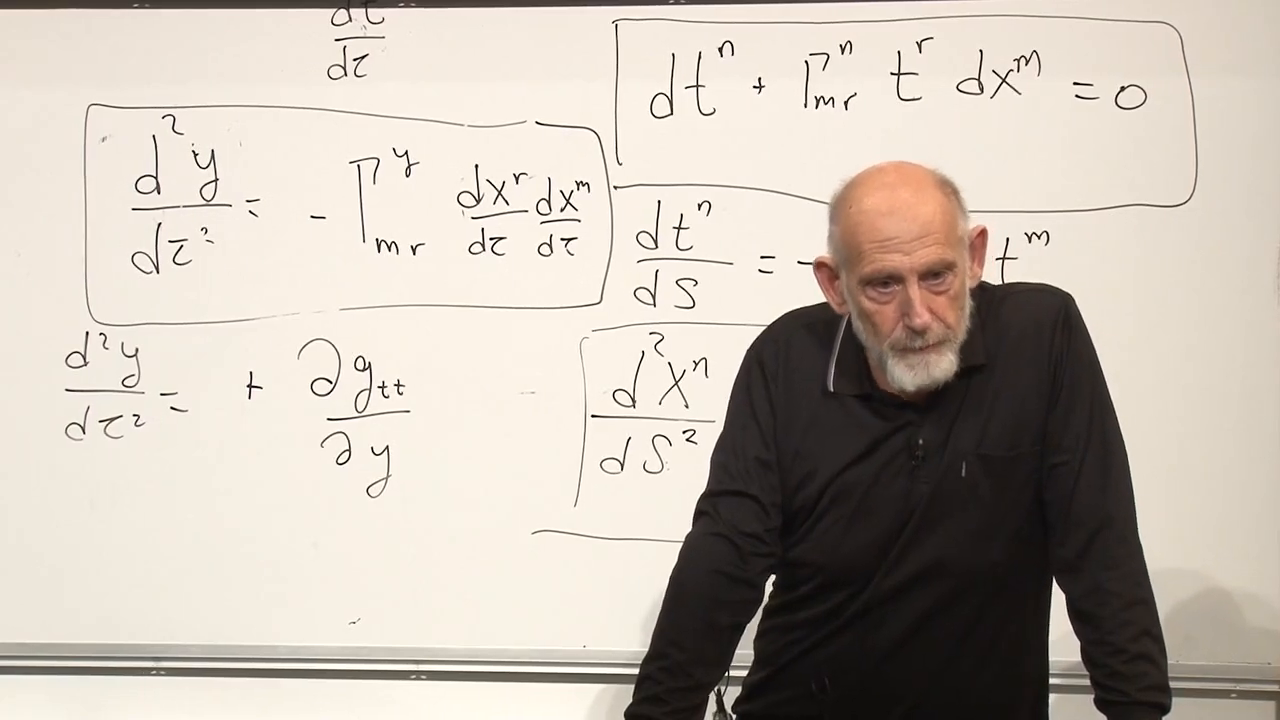
\includegraphics[width=0.90\textwidth]{lecture_04_figure_06.png}\caption{곡면 위의 두 경로를 따라 벡터를 옮기면 마지막 방향이 서로 달라질 수 있다.}\end{figure}

원뿔은 유용한 예다. 꼭짓점에서 떨어진 곳에서는 원뿔을 잘라 펼쳐 평면에 놓을 수 있다. 그런데도 꼭짓점을 둘러싸는 경로를 따라 벡터를 평행이동하면 각결손만큼 회전한 상태로 돌아온다. 꼭짓점을 둥글게 다듬으면 곡률은 유한한 크기로 작은 영역에 퍼진다. 꼭짓점이 완전히 뾰족하다고 이상화하면 곡률이 그 점에 집중된다.

\begin{figure}[htbp]\centering
\includegraphics[width=0.90\textwidth]{lecture_04_figure_07.png}\caption{원뿔 위의 원운동과 이를 잘라 펼친 평면의 표현.}\end{figure}

\subsection{평행이동된 벡터에 관한 질문}

\paragraph{벡터가 모든 곳에서 정의되어 있어야 하는가?}
아니다. 한 점에서 벡터 하나만 정한 뒤, 선택한 곡선을 따라 \eqref{eq:l4-parallel-transport}을 풀면 된다. 벡터장을 정의하는 것은 필수가 아니다. 어떤 영역에 벡터장이 정의되어 있다면, 한 방향을 따라서는 공변적으로 일정하고 다른 방향을 따라서는 그렇지 않을 수 있다.

\paragraph{벡터의 길이는 보존되는가?}
그렇다. \(V^2=g_{mn}V^mV^n\)라고 하자. 곡선을 따라 미분하면
\begin{align}
\frac{D}{d\lambda}\left(g_{mn}V^mV^n\right)
&=
\frac{Dg_{mn}}{d\lambda}V^mV^n
+2g_{mn}V^m\frac{DV^n}{d\lambda}\\
&=0.
\end{align}
계량의 양립성으로 첫째 항이 사라지고, 평행이동 조건으로 둘째 항이 사라진다. 따라서 평행이동된 벡터의 길이와 벡터 사이의 각도는 보존된다.

\paragraph{모든 곡선의 접벡터는 평행이동되는가?}
아니다. 이 질문은 바로 측지선으로 이어진다. 원뿔을 도는 원형 경로의 접벡터는 계속 방향을 바꾼다. 원뿔을 잘라 펼쳤을 때 생기는 직선의 접벡터는 방향을 바꾸지 않는다. 국소적으로 곧은 경로는 두 번째 경로뿐이다.

\section{측지선: 단지 가장 짧은 경로가 아니라 가장 곧은 경로}

측지선에는 서로 관련된 두 가지 설명이 있다. 전역적으로는 길이 또는 고유시간 범함수의 정류 경로다. 국소적으로는 가능한 경로 가운데 가장 곧은 경로다. 여기서 정류라는 말은 중요하다. 기하와 끝점에 따라 그 경로가 전역적인 유일 최솟값을 주지 않을 수 있기 때문이다. 로런츠 시공간에서 시간꼴 측지선은 양의 거리의 최솟값이 아니라 고유시간의 국소 최댓값을 준다.

여기서 필요한 것은 국소적인 설명이다. 지형이 휘는 규모에 비해 작은 자동차를 운전하면서 핸들을 정면에 고정해 두면 측지선을 따라간다. 매입 공간에서 직선처럼 보일 필요는 없다. 곡면 위에서 정의되는 기하에 따르면 곧은 경로다.

\begin{figure}[htbp]\centering
\includegraphics[width=0.90\textwidth]{lecture_04_figure_08.png}\caption{가장 곧은 경로의 정의를 준비하며 곡면 자체에 그린 경로.}\end{figure}

\subsection{접벡터}

곡선을 \(x^m(s)\)라 하고, 호의 길이를
\begin{equation}
ds^2=g_{mn}\,dx^m dx^n.
\end{equation}
라고 하자. 단위 접벡터는
\begin{equation}
t^m=\frac{dx^m}{ds}.
\label{eq:l4-unit-tangent}
\end{equation}
이다. 기하학적으로는 서로 가까운 두 점을 잡아 그 사이의 변위 벡터를 만들고, 두 점 사이의 거리로 나눈 다음 두 점을 서로 접근시킨 극한을 취한다.

\begin{figure}[htbp]\centering
\includegraphics[width=0.90\textwidth]{lecture_04_figure_09.png}\caption{곡선을 따른 변위의 극한으로 정의되는 접선 방향.}\end{figure}

\begin{figure}[htbp]\centering
\includegraphics[width=0.90\textwidth]{lecture_04_figure_10.png}\caption{선요소와 단위 접벡터 \(t^m=dx^m/ds\).}\end{figure}

측지선은 접벡터가 그 자신을 따라 평행이동되는 곡선이다.
\begin{equation}
dt^n+\Gamma^n{}_{mr}t^r\,dx^m=0.
\end{equation}
\(ds\)로 나누고 \(dx^m/ds=t^m\)를 사용하면
\begin{equation}
\frac{dt^n}{ds}
=
-\Gamma^n{}_{mr}t^m t^r.
\end{equation}
마지막으로 \(t^n=dx^n/ds\)를 대입하면
\begin{equation}
\boxed{
\frac{d^2x^n}{ds^2}
+\Gamma^n{}_{mr}
\frac{dx^m}{ds}
\frac{dx^r}{ds}
=0.
}
\label{eq:l4-geodesic}
\end{equation}

\begin{figure}[htbp]\centering
\includegraphics[width=0.94\textwidth]{lecture_04_figure_11.png}\caption{접벡터의 평행이동 법칙과 2계 측지선 방정식.}\end{figure}

\eqref{eq:l4-geodesic}은 이미 뉴턴 역학과 비슷한 모양을 띤다. \(s\)을 적절한 시간 매개변수로 바꾸면 첫째 항은 가속도다. 이어지는 접속 항은 계량만으로 정해지는 질량 단위당 힘처럼 작용한다. 일반상대성이론에서는 이 비유가 실제 물리적 의미를 갖는다. 자유입자는 시공간 측지선을 따르며, 뉴턴 역학에서 중력가속도라고 부른 것은 접속을 통해 나타난다.

\section{리만 거리에서 시공간 고유시간으로}

이제 논의는 곡선 공간에서 시공간으로 옮겨간다. 관성 데카르트 좌표계에서 가까운 두 사건 사이의 고유시간은
\begin{equation}
d\tau^2
=dt^2-dx^2-dy^2-dz^2.
\label{eq:l4-proper-time}
\end{equation}
이다. 강의에서는 다음 식을 사용한다.
\begin{equation}
d\tau^2=-g_{\mu\nu}\,dx^\mu dx^\nu
\label{eq:l4-lecture-sign}
\end{equation}
여기서
\begin{equation}
g_{\mu\nu}
=
\eta_{\mu\nu}
=
\begin{pmatrix}
-1&0&0&0\\
0&1&0&0\\
0&0&1&0\\
0&0&0&1
\end{pmatrix}.
\label{eq:l4-eta}
\end{equation}
이다. 따라서 \eqref{eq:l4-lecture-sign}의 바깥쪽 마이너스 부호는 부호 규약이 대부분 양수인 계량을 \eqref{eq:l4-proper-time}로 바꾼다. 좌표는 다음과 같다.
\begin{equation}
\begin{aligned}
x^\mu&=(t,x,y,z),\\
x^0&=t,\quad x^1=x,\\
x^2&=y,\quad x^3=z.
\end{aligned}
\end{equation}

\begin{figure}[htbp]\centering
\includegraphics[width=0.94\textwidth]{lecture_04_figure_12.png}\caption{고유시간, 시공간 좌표, 대부분 양수인 민코프스키 계량.}\end{figure}

부호수는 불변 정보다. 고윳값 하나는 시간에 해당하는 부호를, 세 개는 공간에 해당하는 부호를 갖는다. 계량 전체에 \(-1\)를 곱하고 모든 규약을 일관되게 조정하면, 똑같이 널리 쓰이는 대부분 음수인 부호 규약을 얻는다. 이런 전반적인 선택은 물리적 내용에 영향을 주지 않는다.

강의에서는 다른 부호수를 가진 공간을 고려한 적이 있는지 묻는다. 수학적으로 다양한 부호수의 의사리만 기하학은 잘 정립되어 있다. 여기서 물리적으로 중요한 점은 더 제한적이다. 관측되는 상대론적 시공간은 시간 방향이 하나인 로런츠 시공간이다. 시간꼴 방향이 더 있다면 인과 구조가 크게 달라지며, 여기서 다루는 물리를 기술하지 못한다.

\begin{figure}[htbp]\centering
\includegraphics[width=0.94\textwidth]{lecture_04_figure_13.png}\caption{평탄한 계량을 \(\eta_{\mu\nu}\)로 나타내기 전에 부호 규약을 확인한다.}\end{figure}

시공간이 평탄하다는 말은 모든 좌표계에서 계량 성분이 반드시 \(\eta_{\mu\nu}\) 형태라는 뜻이 아니다. 그런 성분을 갖는 좌표계가 존재한다는 뜻이다. 곡선좌표나 가속좌표를 사용하면 리만 텐서가 0이어도 계량 성분이 위치에 따라 달라질 수 있다.

\section{같은 좌표 가속도가 강체 운동을 보장하지 않는 이유}

가속하는 승강기에 붙은 좌표계를 구하고자 한다. 첫 번째 생각은 관측자들을 일정한 간격으로 늘어세우고 모두에게 같은 좌표 가속도를 주는 것이다. 하지만 상대론에서는 이 단순한 구성이 강체성을 유지할 수 없다.

\begin{figure}[htbp]\centering
\includegraphics[width=0.92\textwidth]{lecture_04_figure_14.png}\caption{같은 가속도를 주었을 때 이웃한 관측자 사이의 강체성이 유지되는지 살펴보기 위한 관측자들의 일렬 배치.}\end{figure}

한 관성계에서 서로 떨어진 관측자들이 똑같은 가속 프로그램을 따른다면, 변해 가는 순간 정지계에서 관측자 사이의 거리는 일정하게 유지되지 않는다. 관측자들을 잇는 줄은 늘어나 결국 끊어진다. 이는 벨의 우주선 사고실험에서 나타나는 것과 같은 운동학적 긴장이다. 또한 뉴턴 역학에서 일정한 좌표 가속도를 무한히 계속할 수는 없다. 그렇게 하면 결국 빛보다 빠른 속도를 예측하게 된다.

따라서 상대론적으로 강체인 가속 좌표계에서는 위치마다 서로 다른 고유가속도를 사용해야 한다. 지평선이 생길 위치에 가까운 관측자일수록 더 크게 가속하고, 그보다 멀리 있는 관측자는 더 약하게 가속한다. 그러면 순간적으로 함께 움직이는 좌표계에서 관측자 사이의 고유거리를 일정하게 유지할 수 있다. 이것이 한 공간 차원에서의 보른 강체 가속이다.

\section{준비 단계: 유클리드 극좌표}

올바른 구성을 이해하기 위해 먼저 보통의 원에서 시작하는 것이 가장 쉽다. 유클리드 평면에서는
\begin{equation}
x=r\cos\theta,
\qquad
y=r\sin\theta,
\end{equation}
이므로
\begin{equation}
x^2+y^2=r^2,
\qquad
\cos^2\theta+\sin^2\theta=1.
\end{equation}
복소지수 형태는 다음과 같다.
\begin{equation}
\cos\theta=\frac{e^{i\theta}+e^{-i\theta}}{2},
\qquad
\sin\theta=\frac{e^{i\theta}-e^{-i\theta}}{2i}.
\label{eq:l4-euler-trig}
\end{equation}
칠판에서 설명하는 중 사인 공식 분모의 \(i\) 인자가 빠진 것을 발견해 다시 적는다.

\begin{figure}[htbp]\centering
\includegraphics[width=0.94\textwidth]{lecture_04_figure_15.png}\caption{원, 유클리드 극좌표, 그리고 삼각함수의 지수 표현.}\end{figure}

\(r\)가 일정하면 원이 된다. 일정한 각속도로 운동할 때 구심가속도의 크기는 일정하며 항상 안쪽을 향한다. 시공간에서는 쌍곡선이 이에 대응하는 역할을 한다.

\section{민코프스키 시공간의 쌍곡좌표}

삼각함수를 쌍곡함수로 바꾸자.
\begin{equation}
\cosh\omega=\frac{e^\omega+e^{-\omega}}{2},
\qquad
\sinh\omega=\frac{e^\omega-e^{-\omega}}{2},
\end{equation}
여기서
\begin{equation}
\cosh^2\omega-\sinh^2\omega=1.
\label{eq:l4-hyperbolic-identity}
\end{equation}
이다. \(i\) 인자는 없다. 좌표 \(\omega\)은 쌍곡각, 즉 신속도다. 보통의 각과 달리 주기적이지 않으며, 범위는 \(-\infty\)에서 \(+\infty\)까지다.

\begin{figure}[htbp]\centering
\includegraphics[width=0.94\textwidth]{lecture_04_figure_16.png}\caption{시공간 좌표 구성에서 삼각함수를 쌍곡함수로 바꾼다.}\end{figure}

오른쪽 린들러 쐐기에서 새 좌표를 정의하자.
\begin{equation}
x=r\cosh\omega,
\qquad
t=r\sinh\omega,
\qquad
r>0.
\label{eq:l4-rindler-transform}
\end{equation}
그러면
\begin{equation}
x^2-t^2=r^2.
\label{eq:l4-rindler-hyperbola}
\end{equation}
\(r\)을 고정하고 \(\omega\)를 변화시키면 쌍곡선 하나를 따라 움직인다. \(r\)을 증가시키면 공간꼴 방향으로 쌍곡선 무리 사이를 이동하고, \(\omega\)를 증가시키면 시간꼴 방향으로 한 쌍곡선을 따라 앞으로 나아간다.

\begin{figure}[htbp]\centering
\includegraphics[width=0.94\textwidth]{lecture_04_figure_17.png}\caption{좌표변환 \(x=r\cosh\omega\), \(t=r\sinh\omega\)와 그 변환에서 불변인 쌍곡선.}\end{figure}

\begin{figure}[htbp]\centering
\includegraphics[width=0.94\textwidth]{lecture_04_figure_18.png}\caption{강체 가속 관측자 무리를 나타내는 고정 \(r\) 쌍곡선들의 합동.}\end{figure}

\subsection{가속좌표계에서의 계량}

\eqref{eq:l4-rindler-transform}을 미분하면
\begin{align}
dx&=\cosh\omega\,dr+r\sinh\omega\,d\omega,\\
dt&=\sinh\omega\,dr+r\cosh\omega\,d\omega.
\end{align}
\eqref{eq:l4-hyperbolic-identity}를 사용하면 교차항이 상쇄된다.
\begin{align}
d\tau^2
&=dt^2-dx^2\\
&=r^2\,d\omega^2-dr^2.
\label{eq:l4-rindler-metric}
\end{align}
여기에 횡방향을 복원하면 이 강의에서 사용한 고유시간 규약에 따라 \(-dy^2-dz^2\)만 더해진다.

시공간은 여전히 평탄하다. 좌표에 따라 변하는 계수 \(r^2\)는 유클리드 극좌표에서 \(d\theta^2\)에 곱해지는 \(r^2\)만큼이나 곡률의 증거가 되지 않는다.

\subsection{쌍곡선을 따른 고유가속도}

고정된 세계선 \(r=R\)에 대해 \eqref{eq:l4-rindler-metric}은 다음을 준다.
\begin{equation}
d\tau=R\,d\omega.
\end{equation}
그 4-속도는
\begin{equation}
U^\mu
=
\frac{d(t,x)}{d\tau}
=
(\cosh\omega,\sinh\omega),
\end{equation}
이고, 4-가속도는
\begin{equation}
A^\mu
=
\frac{dU^\mu}{d\tau}
=
\frac{1}{R}(\sinh\omega,\cosh\omega).
\end{equation}
이다. 불변 크기는 일정하다.
\begin{equation}
a=\sqrt{A^\mu A_\mu}=\frac{1}{R}
\qquad (c=1).
\label{eq:l4-proper-acceleration}
\end{equation}

\begin{figure}[htbp]\centering
\includegraphics[width=0.90\textwidth]{lecture_04_figure_19.png}\caption{고정된 가속 세계선에서 성립하는 역반지름 법칙 \(a=1/R\).}\end{figure}

단위를 복원하면
\begin{equation}
\boxed{a=\frac{c^2}{R}.}
\label{eq:l4-proper-acceleration-units}
\end{equation}

\begin{figure}[htbp]\centering
\includegraphics[width=0.90\textwidth]{lecture_04_figure_20.png}\caption{단위를 복원하면 \(1/R\)은 \(c^2/R\)이 된다.}\end{figure}

절편 \(R\)이 작을수록 세계선은 더 급하게 휘며, 그 관측자가 느끼는 고유가속도도 더 크다. 더 바깥쪽의 쌍곡선은 덜 휘므로 필요한 가속도도 더 작다. 각 관측자의 가속도는 시간에 따라 일정하지만 관측자마다 가속도는 다르다. 이러한 차이가 바로 관측자 사이의 고유거리를 보존한다.

\subsection{가속좌표계에 관한 질문}

\paragraph{\(R\)는 \(x\)축 절편인가?}
그렇다. \(\omega=0\)일 때 \eqref{eq:l4-rindler-transform}에 따르면 \(t=0\)이고 \(x=R\)이다. 절편은 \eqref{eq:l4-proper-acceleration-units}을 통해 고유가속도를 정한다.

\paragraph{이 구성은 선택한 원점에 의존하는가?}
좌표는 의존한다. 원점을 평행이동하면 점근선이 이동한 또 다른 쌍곡선 무리가 생긴다. 어떤 불변 물리량도 그 선택에 의존하지 않는다. 여기서는 가속좌표계 하나를 의도적으로 선택하고, 그 좌표계에서 관성운동이 어떻게 기술되는지 살펴본다.

\paragraph{고유가속도란 무엇인가?}
관측자와 함께 움직이는 가속도계가 측정하는 가속도다. 공변적으로 쓰면
\begin{equation}
A^\mu=\frac{dU^\mu}{d\tau},
\qquad
U^\mu=\frac{dx^\mu}{d\tau}.
\end{equation}
그 크기는 관측자가 실제로 느끼는 밀어내는 힘이며, 멀리 떨어진 좌표계가 부여하는 좌표가속도 \(d^2x/dt^2\)가 아니다.

\section{극좌표와 쌍곡좌표로 나타낸 평탄한 계량}

지구 근방으로 국소화하기 전에 유클리드 계량과 로런츠 계량을 나란히 살펴보면 유용하다. 평면에서는
\begin{equation}
ds^2=dr^2+r^2d\theta^2,
\qquad
g_{ab}
=
\begin{pmatrix}
1&0\\
0&r^2
\end{pmatrix}.
\label{eq:l4-polar-metric}
\end{equation}
청중의 제안에 따라 구면 인자를 잠깐 도입하지만, 여기서 다루는 것은 구가 아니라 평면이다. \(r^2\) 항은 반지름이 커질수록 같은 각도 간격에 해당하는 원호의 길이가 길어진다는 사실을 나타낸다.

\begin{figure}[htbp]\centering
\includegraphics[width=0.94\textwidth]{lecture_04_figure_21.png}\caption{유클리드 극좌표 계량: 평탄한 평면에서도 위치에 따라 변하는 성분.}\end{figure}

민코프스키 공간에서 이에 대응하는 계량은
\begin{equation}
d\tau^2=r^2d\omega^2-dr^2.
\end{equation}
이다. 두 계량의 성분은 위치에 따라 달라지지만 두 기하학 모두 평탄하다. 좌표에 따른 곡률과 기하학적 곡률은 같은 것이 아니다.

\section{지표면 중력가속도 근방으로 국소화하기}

고유가속도가 지표면 중력가속도 값 \(g\)인 기준 쌍곡선을 하나 선택하자.
\begin{equation}
g=\frac{c^2}{R},
\qquad
R=\frac{c^2}{g}.
\label{eq:l4-earth-radius}
\end{equation}

\begin{figure}[htbp]\centering
\includegraphics[width=0.94\textwidth]{lecture_04_figure_22.png}\caption{기준 쌍곡선을 \(c^2/R=g\)로 선택한다.}\end{figure}

수치로 계산하면
\begin{equation}
R
\simeq
\frac{(3.0\times10^8\ {\rm m\,s^{-1}})^2}
{9.8\ {\rm m\,s^{-2}}}
\simeq
9.2\times10^{15}\ {\rm m}.
\end{equation}
강의에서는 이 값을 \(10^{16}\)미터로 반올림한다. 지표면 중력가속도 \(g\)의 장은 상대론적 척도에서 약하므로, 이에 해당하는 린들러 반지름은 매우 크다.

이제 기준 관측자의 근방에서 작은 영역만 살펴보자. 다음과 같이 국소 높이 \(y\)를 도입한다.
\begin{equation}
r=R+y,
\qquad
dr=dy,
\qquad
|y|\ll R.
\label{eq:l4-local-height}
\end{equation}
토론 중 등식 \(dr=dy\)을 명시적으로 확인했으므로, 공간 항은 \(-dy^2\)로 써야 한다.

\eqref{eq:l4-rindler-metric}를 대입하면
\begin{align}
d\tau^2
&=(R+y)^2d\omega^2-dy^2\\
&=(R^2+2Ry+y^2)d\omega^2-dy^2\\
&=
\left(
1+\frac{2y}{R}+\frac{y^2}{R^2}
\right)
R^2d\omega^2-dy^2.
\label{eq:l4-local-expand}
\end{align}

\begin{figure}[htbp]\centering
\includegraphics[width=0.94\textwidth]{lecture_04_figure_23.png}\caption{\(r=R+y\)을 기준으로 가속계량을 전개한다.}\end{figure}

국소 시간 좌표를 다음과 같이 정의하자.
\begin{equation}
t=R\omega.
\label{eq:l4-local-time}
\end{equation}
그러면
\begin{equation}
d\tau^2
=
\left(
1+\frac{2y}{R}+\frac{y^2}{R^2}
\right)dt^2-dy^2.
\label{eq:l4-local-exact}
\end{equation}

\begin{figure}[htbp]\centering
\includegraphics[width=0.94\textwidth]{lecture_04_figure_24.png}\caption{기준 쌍곡선 근방에서 전개한 뒤 \(t=R\omega\)을 도입한다.}\end{figure}

수십 킬로미터의 수직 이동도 \(R\)에 비하면 작다. 강의에서는 비교를 선명히 보여 주기 위해 대략 24마일 낙하를 예로 든다. 이 거리조차 \(10^{16}\)미터에 비하면 무시할 만큼 작다. 따라서 \(y^2/R^2\)은 \(y/R\)보다 훨씬 작으므로 이차항을 버릴 수 있다.
\begin{equation}
d\tau^2
\simeq
\left(1+\frac{2y}{R}\right)dt^2-dy^2.
\label{eq:l4-local-linear}
\end{equation}

\begin{figure}[htbp]\centering
\includegraphics[width=0.94\textwidth]{lecture_04_figure_25.png}\caption{약한 장 근사로 항을 버리기 전, 전개한 계량과 국소시간 좌표의 치환.}\end{figure}

\(c=1\)인 단위계에서 \eqref{eq:l4-earth-radius}는 \(1/R=g\)을 주므로
\begin{equation}
\boxed{
d\tau^2\simeq(1+2gy)\,dt^2-dy^2.
}
\label{eq:l4-uniform-metric}
\end{equation}

\begin{figure}[htbp]\centering
\includegraphics[width=0.94\textwidth]{lecture_04_figure_26.png}\caption{균일하게 가속하는 승강기의 완성된 국소 계량.}\end{figure}

물리량
\begin{equation}
\Phi(y)=gy
\end{equation}
은 균일한 장에서 질량 단위당 뉴턴 중력 퍼텐셜이다. 따라서
\begin{equation}
d\tau^2\simeq(1+2\Phi)\,dt^2-dy^2
\qquad (c=1).
\label{eq:l4-weak-potential-propertime}
\end{equation}
이다. 강의의 규약 \(d\tau^2=-g_{\mu\nu}dx^\mu dx^\nu\)을 적용하면
\begin{equation}
g_{tt}=-(1+2\Phi).
\label{eq:l4-gtt-potential}
\end{equation}
이 된다. 통상적인 단위계에서 무차원 보정항은 \(2\Phi/c^2\)이다.

시공간은 전혀 휘지 않았다. \eqref{eq:l4-uniform-metric}은 평탄한 린들러 계량을 국소적으로 전개한 결과다. 겉보기 중력은 가속 승강기 안에서 관측되는 관성력이다.

\section{측지선 방정식에서 뉴턴의 운동 법칙으로}

\(gy\)을 퍼텐셜로 보는 해석은 지금까지는 시사적인 수준에 머물렀다. 결정적인 검증은 역학적이다. 계량 \eqref{eq:l4-uniform-metric}에서 자유입자가 \(d^2y/dt^2=-g\)의 가속도로 아래쪽을 향하는가?

고유시간을 매개변수로 삼은 시간꼴 세계선에 대해
\begin{equation}
\frac{d^2x^\nu}{d\tau^2}
+\Gamma^\nu{}_{\mu\rho}
\frac{dx^\mu}{d\tau}
\frac{dx^\rho}{d\tau}
=0.
\label{eq:l4-spacetime-geodesic}
\end{equation}
수직 성분은
\begin{equation}
\frac{d^2y}{d\tau^2}
=
-\Gamma^y{}_{\mu\rho}
\frac{dx^\mu}{d\tau}
\frac{dx^\rho}{d\tau}.
\label{eq:l4-y-geodesic}
\end{equation}

\begin{figure}[htbp]\centering
\includegraphics[width=0.94\textwidth]{lecture_04_figure_27.png}\caption{수직 운동에 적용할 수 있도록 정리한 평행이동 방정식과 그 2계 측지선 형태.}\end{figure}

\subsection{저속 근사}

약한 정적 장에서 천천히 움직이는 입자라면
\begin{equation}
\frac{dt}{d\tau}\simeq1,
\qquad
\left|\frac{dy}{d\tau}\right|\ll1.
\end{equation}
따라서 4-속도의 시간 성분은 대략 1차 크기이고, 공간 성분은 그보다 작다. \eqref{eq:l4-y-geodesic}에 나타나는 곱 가운데 가장 큰 항은 \(\mu=\rho=t\)인 경우다.
\begin{equation}
\frac{d^2y}{d\tau^2}
\simeq
-\Gamma^y{}_{tt}
\left(\frac{dt}{d\tau}\right)^2
\simeq
-\Gamma^y{}_{tt}.
\label{eq:l4-slow-geodesic}
\end{equation}

\begin{figure}[htbp]\centering
\includegraphics[width=0.94\textwidth]{lecture_04_figure_28.png}\caption{느리게 움직이는 입자의 시공간 측지선 방정식에서 \(y\) 성분만 취한다.}\end{figure}

이제 필요한 접속계수를 하나 계산하자. 계량은 대각형이고 \(t\)에 무관하므로
\begin{align}
\Gamma^y{}_{tt}
&=
\frac{1}{2}g^{yy}
\left(
\partial_tg_{yt}
+\partial_tg_{ty}
-\partial_yg_{tt}
\right)\\
&=
-\frac{1}{2}\partial_yg_{tt},
\label{eq:l4-gamma-ytt}
\end{align}
강의의 대부분 양수인 텐서 부호 규약에서는 \(g^{yy}=1\)이기 때문이다.

\begin{figure}[htbp]\centering
\includegraphics[width=0.94\textwidth]{lecture_04_figure_29.png}\caption{\(y,t,t\) 성분으로 줄인 크리스토펠 공식.}\end{figure}

\eqref{eq:l4-slow-geodesic}과 \eqref{eq:l4-gamma-ytt}을 결합하면
\begin{equation}
\frac{d^2y}{d\tau^2}
\simeq
\frac{1}{2}\partial_yg_{tt}.
\label{eq:l4-accel-gtt}
\end{equation}
\eqref{eq:l4-gtt-potential}에서
\begin{equation}
\partial_yg_{tt}
=
-2\partial_y\Phi
=
-2g.
\end{equation}
따라서
\begin{equation}
\boxed{
\frac{d^2y}{d\tau^2}=-g.
}
\label{eq:l4-newton-result}
\end{equation}
같은 저속 근사에서 \(t\simeq\tau\)이므로, 이는 다음 식과도 같다.
\begin{equation}
\frac{d^2y}{dt^2}=-g.
\end{equation}

\begin{figure}[htbp]\centering
\includegraphics[width=0.94\textwidth]{lecture_04_figure_30.png}\caption{부호를 차례로 정리하면 \(g_{tt}\)의 \(y\) 미분에서 가속도 \(-g\)가 나온다.}\end{figure}

더 일반적으로 뉴턴 역학이 성립하는 영역에서는
\begin{equation}
\boxed{
\begin{aligned}
g_{tt}&=-(1+2\Phi),\\
\frac{d^2x^i}{dt^2}&=-\partial_i\Phi
\end{aligned}
}
\qquad(c=1).
\label{eq:l4-newton-general}
\end{equation}
단위를 복원하면 계량의 보정항은 \(2\Phi/c^2\)이고, 가속도는 \(-\boldsymbol{\nabla}\Phi\)이다.

이 계산은 별도의 중력장 대신 계량이 핵심 대상인 이유를 보여 준다. 자유입자는 그저 시공간 측지선을 따른다. 가속 실험실에 맞춘 좌표계에서는 그 측지선이 좌표상으로 휘어 있으며, 보통 이를 중력 탓으로 돌린다.

\subsection{린들러 원점 선택에 관한 질문}

기준 쌍곡선을 평행이동해 점근선과 절편이 다른 곳에 오도록 할 수 있었을까? 그렇다. 적절히 평행이동한 원점마다 그에 대응하는 균일 가속 좌표계가 존재한다. 승강기에 비유하면, 이 선택들은 어느 한순간 바닥이 서로 다른 위치에 있는 승강기들을 고르는 것과 같다.

국소적인 결과는 특별한 원점에 의존하지 않는다. 고유가속도 \(g\)인 기준 관측자를 선택하면 \(y\)은 그 관측자를 기준으로 한 높이를 나타내며, 그 근방의 계량은 \eqref{eq:l4-uniform-metric}의 형태를 띤다. 임의로 정한 좌표계가 바닥을 어디라고 기술할지를 정하지만, 불변 곡률을 만들어 내지는 않는다.

\section{크리스토펠 기호가 텐서일 수 없는 이유}

강의 후 토론에서는 복습 중 처음 다루었던 쟁점으로 돌아간다. 원래의 관성좌표계에서는
\begin{equation}
g_{\mu\nu}=\eta_{\mu\nu},
\qquad
\partial_\rho\eta_{\mu\nu}=0,
\qquad
\Gamma^\mu{}_{\nu\rho}=0.
\end{equation}
자유입자는 직선 운동을 하며 중력은 작용하지 않는다.

가속 좌표계에서는 동일한 평탄 시공간의 계량 성분이 위치에 따라 달라집니다. 크리스토펠 기호는 영이 아니며, 동일한 관성 궤적도 휘어진 것처럼 나타납니다. 입자는 승강기 바닥 쪽으로 떨어지는 것처럼 보입니다.

\(\Gamma^\mu{}_{\nu\rho}\)가 텐서라면 이는 불가능합니다. 한 좌표계에서 영인 텐서는 모든 좌표계에서 영입니다. 반면 접속은 좌표 변환을 할 때 비균질 항을 얻으므로, 관성 좌표계에서는 영이고 가속 좌표계에서는 영이 아닐 수 있습니다. 등가 원리가 요구하는 바가 바로 이것입니다:
\begin{equation}
\text{accelerated frame}
\quad\longleftrightarrow\quad
\text{local gravity}.
\end{equation}

곡률은 다르게 거동합니다. 리만 텐서는 텐서입니다. 관성 좌표계에서 영이면 가속 좌표계에서도 영입니다:
\begin{equation}
R^\mu{}_{\nu\rho\sigma}=0.
\end{equation}
따라서 크리스토펠 기호는 좌표계에 따라 달라지는 중력의 힘을 나타내고, 곡률은 좌표 변환으로 없앨 수 없는 불변의 조석 효과를 포착합니다.

\section{균일 퍼텐셜에서 슈바르츠실트 계량의 미리보기로}

가속 승강기에는 중력을 만드는 물질도 곡률도 없다. 그런데도 약한 장의 관계식 \eqref{eq:l4-newton-general}은 실제 구형 질량이 만드는 장에서 무엇을 찾아야 할지 시사한다. 질량 \(M\)의 바깥에서 뉴턴 퍼텐셜은
\begin{equation}
\Phi(r)=-\frac{GM}{r}.
\label{eq:l4-newton-potential}
\end{equation}
이다. 이를 약한 장에서의 시간 성분에 대입하면
\begin{equation}
g_{tt}
\simeq
-\left(1-\frac{2GM}{r}\right)
\qquad(c=1).
\label{eq:l4-schwarzschild-preview}
\end{equation}
을 얻는다. 칠판 토론 중 퍼텐셜의 부호를 바로잡는다. 인력이 되려면 퍼텐셜은 음수여야 하며, \(r\)이 무한대로 갈 때 아래쪽에서 0에 접근해야 한다.

\begin{figure}[htbp]\centering
\includegraphics[width=0.94\textwidth]{lecture_04_figure_31.png}\caption{뉴턴 퍼텐셜을 시간-시간 계량 성분에 대입하면 \(1-2GM/r\) 인자가 나타난다.}\end{figure}

이 계량 성분은 다음에서 영이 됩니다:
\begin{equation}
r=2GM
\qquad(c=1),
\end{equation}
단위를 복원하면 다음과 같습니다:
\begin{equation}
r_s=\frac{2GM}{c^2}.
\end{equation}
이것이 슈바르츠실트 반지름입니다. 이 특정 계량 성분이 영이 되는 것은 지평선의 전조입니다.

이 논증은 유도 과정이 아니라 의도적으로 미리 보여 주는 설명으로 제시된다. 약한 장 근사만으로는 \(r=2GM/c^2\) 부근의 정확한 슈바르츠실트 해를 확립할 수 없다. 바로 그곳에서는 보정항이 더 이상 작지 않기 때문이다. 완전한 해에는 자명하지 않은 방사 성분도 포함되어야 하며, 아인슈타인 장방정식을 만족해야 한다. 이 방정식들은 아직 도입하지 않았다. 여기까지의 논의가 보여 주는 것은 올바른 구조적 단서와 질적으로 새로운 현상이 나타나야 하는 규모다.

\section{수업 중 질문과 정정}

\subsection{쌍곡각은 보통의 각처럼 작용하는가?}

아니다. 두 변수 모두 일정한 반지름의 곡선족을 따라 운동을 매개변수화하지만, \(\theta\)는 주기적인 반면 rapidity \(\omega\)는 실수 전체의 값을 갖는다. 여기서 각이라는 말은 회전과 로런츠 부스트 사이의 대수적 유사성을 가리킬 뿐, 그 양이 \(0\)과 \(2\pi\) 사이로 제한된다는 뜻은 아니다.

\subsection{크지 않은 가속도에 왜 엄청나게 큰 R이 필요한가?}

관계식 \(a=c^2/R\)에는 큰 상대론적 척도 \(c^2\)가 들어 있다. 가속도를 겨우 \(10\ {\rm m\,s^{-2}}\)로 만들려면 \(R\)가 \(10^{16}\)미터 정도여야 한다. 이것은 지구에 딸린 새로운 물리적 거리가 아니다. 민코프스키 도표에서 쌍곡선 세계선의 곡률 반지름을 길이 단위로 나타낸 것이다.

큰 반지름은 유용한 뉴턴 역학적 구간도 보장한다. 실험실에서 다루는 시간과 거리 동안 속도는 \(c\)보다 훨씬 낮게 유지되고, 가속도는 장치 전체에서 거의 변하지 않으며, \(t\)는 고유시간과 거의 다르지 않다.

\subsection{겉보기 중력장은 실제로 존재하는가?}

고정된 린들러 위치에 붙들려 있는 관찰자에게는 가속도계가 읽는 값으로서 실재하지만, 불변적인 곡률은 아니다. 관찰자를 놓아주면 가속도계는 그 결과로 이어지는 관성 측지선을 따라 영을 가리킨다. 충분히 작은 자유낙하 실험실에서는 균일장을 국소적으로 제거할 수 있다. 유한한 영역에 걸쳐 제거할 수 없는 것은 조석장이며, 이는 영이 아닌 곡률로 나타난다.

\subsection{힘을 계산하는 과정에서 무엇을 바로잡았는가?}

계산 도중 부호 몇 가지와 1/2 계수를 확인한다. 강의에서 사용하는 규약에 따른 신뢰할 수 있는 전개는 다음과 같다.
\begin{equation}
\begin{aligned}
g_{tt}&=-(1+2gy),\\
\Gamma^y{}_{tt}&=-\frac12\partial_yg_{tt}=g,\\
\frac{d^2y}{d\tau^2}&=-\Gamma^y{}_{tt}=-g.
\end{aligned}
\end{equation}
규약을 명시하면 칠판 앞에서 잠시 부호를 망설인 일이 물리적 모호성으로 이어지는 것을 막을 수 있다.

\section{확립된 결과}

강의는 미분기하학에서 시작해 뉴턴 역학에서 낙하하는 물체로 끝난다. 핵심 단계는 다음과 같다.
\begin{enumerate}
\item 공변미분은 좌표 기저가 변할 때 텐서를 비교한다.
\item 평행이동은 선택한 경로를 따라 공변 변화가 0인 것을 뜻한다.
\item 측지선에서는 그 접벡터 자체가 평행이동된다.
\item 자유 입자는 시공간의 측지선을 따른다.
\item \(r\)가 고정된 쌍곡선들은 상대론적으로 강체인 가속 좌표계를 이룬다.
\item 이들의 고유가속도는 \(a=c^2/r\)이므로 위치에 따라 달라져야 한다.
\item 가속도 \(g\)를 갖는 기준 세계선 부근에서 평탄한 계량은 다음과 같다.
\begin{equation}
d\tau^2\simeq(1+2gy)\,dt^2-dy^2
\qquad(c=1).
\end{equation}
\item 측지선 방정식은 다음과 같이 환원된다.
\begin{equation}
\frac{d^2y}{dt^2}=-g.
\end{equation}
\end{enumerate}

따라서 등가원리는 엘리베이터와 중력 사이의 비유에 그치지 않는다. 계량과 그 접속이 변환되는 방식에 등가원리가 담겨 있다. 평탄한 시공간을 가속 좌표계로 나타내면 균일한 중력처럼 보이는 힘이 생길 수 있지만, 곡률은 0으로 남는다.

마지막으로 살펴본 외삽은 균일장을 넘어선다. \(\Phi=gy\)를 \(\Phi=-GM/r\)로 바꾸면 구대칭 계량의 시간 성분에 특징적인 인자 \(1-2GM/r\)가 나타나고, 슈바르츠실트 척도가 드러난다. 그러나 전체 기하를 결정하려면 장방정식이 필요하다. 다음 강의에서는 이 문제를 다룬다.
